\documentclass{beamer}

\usepackage{tikz-cd}

\usepackage{amsthm}
\usepackage[utf8]{inputenc}
\usepackage[T2A]{fontenc}
% \usepackage[svgnames]{xcolor}
% \usepackage[pdftex]{graphicx}
\usepackage{
  amsfonts
 ,amsmath
 ,amssymb
 ,caption
 ,epigraph
 ,lipsum
 ,mathtools
 ,hyphenat
 ,tensor
 ,todonotes
 ,stackrel
 ,savesym
 ,setspace
 ,stmaryrd
 ,tikz-cd
 ,verbatim
 ,calligra}

\usepackage{tikz}
	\usetikzlibrary{calc}
	\usetikzlibrary{matrix,arrows}

\usepackage[all,2cell]{xy}\UseAllTwocells

\usepackage[
 ,sort
 ,numbers
]{natbib}

% \usepackage[%
%    hyperfootnotes=true
%   ,colorlinks%
%   ,citecolor=blue!40!black%
%   ,linkcolor=blue!40!black%
%   ]{hyperref}
\usepackage{mathabx,esint}
\restoresymbol{ABX}{second}

\usepackage{CJKutf8}

% \usepackage[%
% 	left=4cm
% 	,right=4cm
% 	,top=4cm
% 	,bottom=6cm%
% ]{geometry}
%per le formule nei titoli
%-------------------------------------------------------------------------
\makeatletter
\g@addto@macro\bfseries{\boldmath}
\makeatother
%-------------------------------------------------------------------------

\renewcommand{\textbf}[1]{\text{\fontseries{b}\selectfont{\upshape #1}}}

\def\CAT{\mathbf{CAT}}
\def\Cat{\mathbf{Cat}}
\def\caat{\mathbf{cat}}
\def\Set{\mathbf{Set}}
\def\Ab{\mathbf{Ab}}


\newcommand{\arXivPreprint}[1]{\href{http://arxiv.org/abs/#1}{arXiv:#1} preprint}

\newlength{\seplen}
\setlength{\seplen}{5pt}
\newlength{\sepwid}
\setlength{\sepwid}{.4pt}
\def\firstblank{\,\rule{\seplen}{\sepwid}\,}
\def\secondblank{\firstblank\llap{\raisebox{2pt}{\firstblank}}}

% \DeclareDocumentEnvironment{enumtag}{m}{
% 	\begin{enumerate}[label=\textsc{#1}\oldstylenums{\arabic*}),ref=\textsc{#1}\oldstylenums{\arabic*}]
% 		}
% 		{
% 	\end{enumerate}
% }

\def\op{\text{op}}
\def\co{\text{co}}
\def\coop{\text{coop}}

\newcommand{\celtag}[2][dr]{\ar[#1,white, "#2"{black,description}]}

\def\ran{\mathrm{ran}}
\def\Ran{\mathrm{Ran}}
\def\RAN{\textsc{Ran}}
\def\lan{\mathrm{lan}}
\def\Lan{\mathrm{Lan}}
\def\Yan{\mathrm{Yan}}
\def\LAN{\textsc{Lan}}
\def\rift{\mathrm{rift}}
\def\Rift{\mathrm{Rift}}
\def\RIFT{\textsc{Rift}}
\def\leeft{\mathrm{lift}}
\def\Lift{\mathrm{Lift}}
\def\LIFT{\textsc{Lift}}
\def\Nat{\textsf{Nat}}

\newcommand{\psh}[2][\Set]{[{#2}^\op,#1]}

\DeclareMathOperator{\colim}{colim}
\def\Mod{\textsf{Mod}}
\def\jb{\smalltriangleleft}

\usepackage{turnstile}
\newcommand{\adjunct}[2]{\nsststile{#2}{#1}}

\let\xto\xrightarrow
\def\sb{{}^\bullet\kern-.1em}
\tikzset{commutative diagrams/.cd,arrow style=tikz,diagrams={>=stealth'}}
\def\To{\Rightarrow}
\def\llambda{\text{л}}

\newcommand{\Nearrow}{\rotatebox[origin=c]{45}{$\Rightarrow$}}
\newcommand{\Nwarrow}{\rotatebox[origin=c]{135}{$\Rightarrow$}}
\newcommand{\Searrow}{\rotatebox[origin=c]{-45}{$\Rightarrow$}}
\newcommand{\Swarrow}{\rotatebox[origin=c]{225}{$\Rightarrow$}}
\newcommand{\Sarrow}{\rotatebox[origin=c]{-90}{$\Rightarrow$}}
\newcommand{\Narrow}{\rotatebox[origin=c]{90}{$\Rightarrow$}}
\def\VCAT{\cV\text{-}\CAT}
\def\Spec{\text{Spec}}
\newcommand{\adjani}[2]{
\xymatrix@C=7mm{ A \ar@<4pt>[r]^{#1} \ar@{}[r]|\perp  & \ar@<4pt>[l]^{#2} B }}
\def\Prof{\mathsf{Prof}}
\def\yose{\left\{\begin{smallmatrix}
		\mathrm{yosegi} \\ \mathrm{boxes}
	\end{smallmatrix}\right\}}
\def\yone{\left\{\begin{smallmatrix}
		\mathrm{cocomplete}\\\mathrm{Yoneda} \\ \mathrm{structures}
	\end{smallmatrix}\right\}}
\def\equ{\left\{\begin{smallmatrix}
		\mathrm{Yoneda} \\ \mathrm{equipments}
	\end{smallmatrix}\right\}}
\def\reladjL#1{\tensor*[^{}_{#1}]{\dashv}{}}
\def\cf{\textsf{cf}}
\newcommand{\crc}{\cdot}
\def\dual{\lor}
\def\odot{\mathop{\ooalign{$\circ$\cr$\hfil\cdot\hfil$}}}
\newcommand{\deduction}[4]{\begin{array}{c} #1 \to #2 \\ \hline #3 \to #4 \end{array}}
\setlength{\epigraphwidth}{0.6\textwidth}


\newcommand{\RescaleSymbol}[2][.75]{\mathbin{\vcenter{\hbox{\scalebox{#1}{$#2$}}}}}
\def\myboxmin{\RescaleSymbol[.6]{\boxminus}}

\def\Kl{\boldsymbol K\kern-.22em\raisebox{-.06em}{$\boldsymbol\ell$}}
\usepackage{xparse}

\ExplSyntaxOn
\NewDocumentCommand{\makeabbrev}{mmm}
 {
  \yoruk_makeabbrev:nnn { #1 } { #2 } { #3 }
 }

\cs_new_protected:Npn \yoruk_makeabbrev:nnn #1 #2 #3
 {
  \clist_map_inline:nn { #3 }
   {
    \cs_new_protected:cpn { #2 } { #1 { ##1 } }
   }
 }
\ExplSyntaxOff

\makeabbrev{\textbf}{b#1}{b,c,d,e,g,h,i,j,k,l,m,n,o,p,q,r,t,u,v,w,x,y,z,%
              B,C,D,E,G,H,I,J,K,L,M,N,O,P,Q,R,T,U,V,W,X,Y,Z}

\makeabbrev{\boldsymbol}{bs#1}{%
    a,b,c,d,e,f,g,h,i,j,k,l,m,n,o,p,q,r,s,t,u,v,w,x,y,z,%
    A,B,C,D,E,F,G,H,I,J,K,L,M,N,O,P,Q,R,S,T,U,V,W,X,Y,Z}

\makeabbrev{\mathsf}{sf#1}{a,b,c,d,e,f,g,h,i,j,k,l,m,n,o,p,q,r,s,t,u,v,w,x,y,z,%
                           A,B,C,D,E,F,G,H,I,J,K,L,M,N,O,P,Q,R,S,T,U,V,W,X,Y,Z}
\makeabbrev{\mathfrak}{f#1}{a,b,c,d,e,f,g,h,j,k,l,m,n,o,p,q,r,s,t,u,v,w,x,y,z,%
                             A,B,C,D,E,F,G,H,I,J,K,L,M,N,O,P,Q,R,S,T,U,V,W,X,Y,Z}
\makeabbrev{\mathcal}{c#1}{A,B,C,D,E,F,G,H,I,J,K,L,M,N,O,P,Q,R,S,T,U,V,W,X,Y,Z}
\makeabbrev{\mathbb}{s#1}{A,B,C,D,E,F,G,H,I,J,K,L,M,N,O,P,Q,R,S,T,U,V,W,X,Y,Z}


\newcommand{\mymu}{\boldsymbol{\mu}}
\newcommand{\myeta}{\boldsymbol{\eta}}

\setbeamertemplate{itemize items}{$\bullet$}

\author[Fosco Loregian]{%
	Fosco Loregian \\ 
	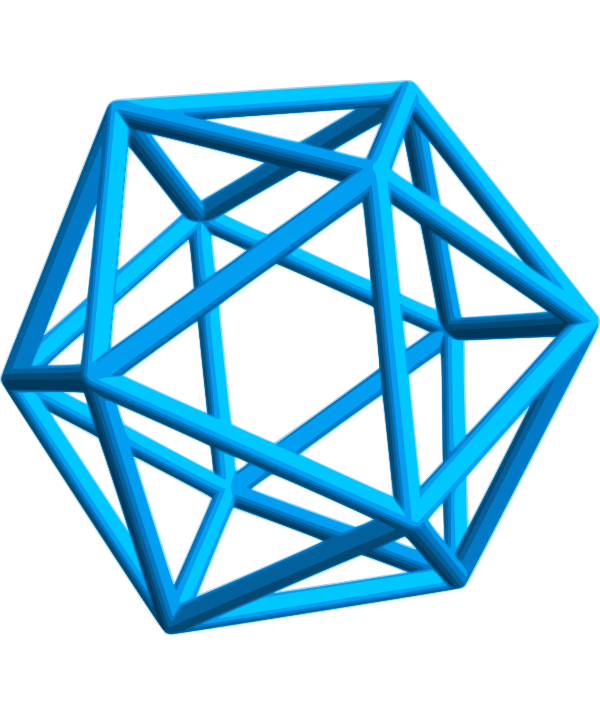
\includegraphics[scale=.05]{MPIM.png} \\ 
	Max Planck Institute for Mathematics%
}
\title[Unicity]{On the unicity of the formal theory of categories}
\date{February 4, 2019}
\usetheme{CambridgeUS}
\setbeamertemplate{navigation symbols}{}
\begin{document}

\begin{frame}
	\maketitle
\end{frame}

\begin{frame}
	\begin{itemize}
		\item<1-> All I'm about to say is \alert{arXiv1901.01594}
		\item<2-> This circle of ideas is young; feel free to comment and join
		\item<3-> Our original motivation was to investigate the \alert{formal category theory of derivators }.
	\end{itemize}
\end{frame}

\begin{frame}{Plan of the talk}
	\begin{itemize}
		\item<1-> Fast and painless intro to formal category theory
		\item<2-> Setting the stage: bits of 2-category theory I'll need along the discussion
		\item<3-> the current state of art: Yoneda lemma VS bimodules
		\item<4-> \alert{Main theorem}: ``Yoneda structures $\sim$ proarrow equipments.''
		\item<5-> Examples:
		      \begin{itemize}
			      \item Representable Yoneda structure
			      \item Two-sided Yoneda structure
			      \item Isbell duality and its generalizations
		      \end{itemize}
		\item<6-> An open and motivating problem: derivators.
	\end{itemize}
\end{frame}

\begin{frame}
	\centering\Huge Introduction
\end{frame}
\begin{frame}
	\begin{itemize}
		\item Formal category theory is a branch of 2-category theory
		\item it serves to axiomatize the \alert{structural part} of category theory
	\end{itemize}
	\onslide<2->
	In the words of John Gray
	\begin{block}{1.}
		<<The purpose of category theory is to try to describe certain general
		aspects of the structure of mathematics. Since category theory
		is also part of mathematics, this categorical type of description
		should apply to it as well as to other parts of mathematics.>>
	\end{block}
	\onslide<3->
	\begin{block}{2.}
		<<The category of small categories, $\Cat$, is a ``2-category with properties''; one should attempt to identify those properties that enable one to do the ``structural parts of category theory''.>>
	\end{block}
\end{frame}

\begin{frame}
	1. reads as ``category \alert{theory} is a \alert{theory} we can interpret in different contexts''; these contexts are 2-categories.\onslide<2->

	\medskip 
	2. reads as ``our task is unravel the properties enabling to treat an abstract 2-category $\cK$ as if it were $\Cat$''.

	\vspace*{1cm}
	\onslide<3->
	Not a new idea:
	\begin{itemize}
		\item cf. \alert{topos theory}: treat  a category$\cE$ as if it were $\Set$;
		\item cf. \alert{categorical algebra}: treat a category $\cA$ as if it were $\text{Alg}(\sT)$;
		\item cf. \alert{homological algebra}: treat a category $\cC$ as if it were $\text{Ch}(\cA)$;
	\end{itemize}
\end{frame}

\begin{frame}
	Perhaps surprisingly though, the bare structure of a 2-category does not suffice to embody ``all'' category theory in a formal way. (In short: there are features of 2-category theory induced by the fact that 2-$\bf Cat$ is a 3-category)

	\bigskip\onslide<+->
	Sure you can do many things:
	\begin{itemize}
		\item<+-> adjunctions: pairs of 1-cells $f : X \leftrightarrows Y : g$ with \alert{co/unit};
		\item<+-> monads: endo-1-cells $t : A\to A$ with \alert{multiplication} and \alert{unit};
		\item<+-> Kan extensions;
		\item<+-> internal fibrations\dots
	\end{itemize}
\end{frame}
\begin{frame}
	but many other important things are missing:
	\bigskip
	\begin{itemize}
		\item<+-> a ``pointwise'' formula to compute Kan extensions
		\item<+-> equivalent characterization of adjunctions: $Y(f,1)\cong X(1,g)$
		\item<+->[Y)] the \alert{Yoneda lemma} (representably and fibrationally)
		\item<+->[E)] a \alert{calculus of modules} (every bimodule $M : A^\lor\times B\to S$ can be straightened to a fibration over $A^\lor\times B$)
	\end{itemize}
	\onslide<+->
	\begin{block}{Idea}
		Take a 2-category $\cK$, and take Y) and E) very seriously.
	\end{block}
\end{frame}
\begin{frame}
	\begin{block}{Y): Yoneda structures}
		\begin{itemize}
			\item<1-> Category theory is the class of corollaries of Yoneda lemma.
			\item<2-> A \emph{Yoneda structure} imposes on $\cK$ enough structure so that every ``small'' object $A$ has a ``Yoneda embedding'' $y_A : A\to PA$.
			\item<3-> Formally encode the Yoneda lemma in universal properties of certain diagrams
			      \[
				      \xymatrix{
					      &A \ar[dr]^f\ar[dl]_{y_A}&\\
					      PA \urlowertwocell<\omit>{<3>\quad\chi^f}&&\ar[ll]^{B(f,1)} B
				      }
			      \]
			      representing \alert{$f$-nerves}.
		\end{itemize}
	\end{block}
\end{frame}
\begin{frame}
	\begin{block}{E): proarrow equipments}
		\begin{itemize}
			\item<1-> Category theory is the theory of multi-object monoids.
			\item<2-> And monoids are well-known for their irresistible tendency to act on objects!
			\item<3-> This leads to the notion of \alert{$C$-$D$-bimodule} as a functor $C^\op\times D\to Set$. All such bimodules live in a bicategory $Mod$, and there is an embedding \[p : Cat \hookrightarrow Mod\] such that every $f\in Cat$ has a right adjoint when embedded in $Mod$.
			\item<4-> Every such $p : \cK \to \overline{\cK}$ \alert{equips $\cK$ with proarrows}.
		\end{itemize}
	\end{block}
\end{frame}
\begin{frame}
	The main theorem of this talk is an equivalence between a certain class of Yoneda structures and a certain class of proarrow equipments:
	\[
		\notag
		\alt<2->{\begin{tikzcd}[ampersand replacement=\&]
				\& {\color{red} \yose} \arrow[Rightarrow,rd,red] \&  \\
				{\yone} \arrow[Rightarrow,ru,red] \&  \& {\equ} \arrow[Rightarrow,ll]
			\end{tikzcd}}{\begin{tikzcd}[ampersand replacement=\&]
				\& {\color{white} \yose}  \&  \\
				{\yone} \&  \& {\equ} \arrow[Rightarrow,ll]
			\end{tikzcd}}
	\]
	\onslide<3->
	What allows to pass from YS to E is the notion of a \alert{yosegi}, a certain special kind of 2-monad.
\end{frame}
\begin{frame}
	\Huge \centering Preliminaries
\end{frame}
\begin{frame}{2-dimensional universality}
	The main 2-dimensional universal constructions we are interested in%: the definition of Yoneda structure \centering relies on the notion of left extension (and on a minor note, left lifting). %Even though all four universals are on the same ground conceptually, extensions are undoubtedly far more common, and they are psycologically easier to grasp precisely by their ubiquity.
	\[
		\begin{array}{|c|c|}\hline
			\xymatrix{
			A \ar@{}[dr]|(.3){\Swarrow\eta}\ar[d]_g \ar[r]^f        & B                                      \\
			C \ar@{.>}[ur]_{\Lan_gf}                                & {\tiny \deduction{\Lan_gf}{h}{f}{hg}}
			}
			                                                        &
			\xymatrix{
			{\tiny \deduction{\Lift_gf}{h}{f}{gh}}                  & C\ar[d]^g                              \\
			B\ar[r]_f \ar@{.>}[ur]^{\Lift_gf}                       & \ar@{}[ul]|(.3){\Nearrow\eta} A
			}                                                                                                \\ \hline
			%%%
			\xymatrix{
			A \ar@{}[dr]|(.3){\Nearrow\varepsilon}\ar[d]_g \ar[r]^f & B                                      \\ C
			\ar@{.>}[ur]_{\Ran_gf}                                  & {\tiny \deduction{hg}{f}{h}{\Ran_gf}}
			}
			                                                        &
			\xymatrix{
			{\tiny \deduction{h}{\Rift_gf}{gh}{f}}                  & C\ar[d]^g                              \\ B\ar[r]_f
			\ar@{.>}[ur]^{\Rift_gf}                                 & \ar@{}[ul]|(.3){\Swarrow\varepsilon} A
			}                                                                                                \\ \hline
		\end{array}
	\]
	{\onslide<2->\alert{pointwise}\dots} \hspace{\fill} {\onslide<3->\dots\alert{absolute}}
\end{frame}
\begin{frame}
	\begin{block}{Proposition (formal description of adjoints)}
		The following conditions are equivalent, for a pair of 1-cells \(f : A \leftrightarrows B : g\)
		\begin{itemize}
			\item<+->  $f \dashv g$ with unit $\eta$ and counit $\epsilon$;
			\item<+->  The pair $\langle g,\eta\rangle$ exhibits the absolute Lan of $1$ along $f$
			\item<+->  The pair $\langle g,\eta\rangle$ exhibits the Lan of $1$ along $f$, and $f$ preserves it.
		\end{itemize}
	\end{block}
	\onslide<+->	(Exercise: properly dualize this statement)
\end{frame}
\begin{frame}
	A bit of coend calculus:
	\begin{block}{Proposition (ninja Yoneda lemma)}
		For every presheaf $F : \cC\to \Set$, it holds
		\[F(X) \cong \int_{A}FX^{\hom(A,X)} \qquad
			F(X) \cong \int^A FA \times\hom(X,A)\]
		naturally in $X$.
	\end{block}
	\onslide<2->
	\begin{block}{Proposition (pointwise Kan extensions)}
		For a diagram $\cC \xleftarrow{G} \cA \xto{F}\cB$, it holds
		\[\Lan_GF(X)\cong \int^A \hom(GA,X)\times FA\]
		naturally in $X$.
	\end{block}
\end{frame}
\begin{frame}
	\Huge\centering Yoneda structures
\end{frame}
\begin{frame}
	Let $\cK$ be a 2-category; a \alert{Yoneda structure} on $\cK$ is made of\onslide<2->
	\begin{itemize}
		\item \alert{Yoneda data}
		      \begin{itemize}
			      \item<3-> An \alert{ideal} of admissible arrows $\fJ$
			            \begin{center}
				            \scriptsize identity morphisms in the ideal determine admissible \emph{objects}.
			            \end{center}
			      \item<4-> a family of morphisms $y_A : A\to \bsP A$ one for each admissible object $A$
			            \begin{center}
				            \scriptsize beware! $\bsP A$ is only syntactic sugar. It has no meaning whatsoever.
			            \end{center}
			      \item<5-> A family of triangles
			            \[
				            \xymatrix{
					            &A \ar[dr]^f\ar[dl]_{y_A}&\\
					            PA \urlowertwocell<\omit>{<3>\quad\chi^f}&&\ar[ll]^{B(f,1)} B
				            }
			            \]
			            filled by a 2-cell $\chi : y_A \to B(f,f) =: B(f,1)\crc f$.
		      \end{itemize}
	\end{itemize}
\end{frame}
\begin{frame}
	\begin{itemize}
		\item subject to \alert{Yoneda axioms}
		      \begin{itemize}
			      \item<2->  The pair $\langle B(f,1), \chi^f\rangle$ exhibits the pointwise left extension $\Lan_fy_A$.
			      \item<3->  The pair $\langle f, \chi^f\rangle$ exhibits the absolute left lifting $\LIFT_{B(f,1)}y_A$ (\alert{shortly, $f\reladjL{y_A} B(f,1)$}).
			      \item<4->  The pair $\langle 1_{\bsP A}, 1_{y_A} \rangle$ exhibits the pointwise left extension $\Lan_{y_A}y_A$ (\alert{shortly, `the Yoneda embedding is dense'}).
			      \item<5->  Given a pair of composable 1-cells $A \xto{f} B\xto{g} C$, the
			            pasting of 2-cells
			            $$ \footnotesize \begin{tikzcd}[column sep=large, row sep=large,ampersand replacement=\&] A\ar[d, "f"']\ar[rr, "y_A"{name=yonA}] \&\& \bsP A\\ B \ar[r, "y_B"{name=yonB}]\ar[d, "g"'] \& \bsP B\ar[ur, "\bsP f"']\\ C\ar[ur, "{C(g,1)}"'] \ar[from=yonA, to=yonB, shorten >=2mm, shorten <=4mm, Rightarrow, "\chi^{y_B f}"] \ar[from=yonB, shorten >=4mm, shorten <=4mm, Rightarrow, "\chi^g"] \end{tikzcd} $$
			            exhibits the pointwise extension $\Lan_{gf}y_A = C(gf,1)$ (\alert{shortly, $\bsP$ is a functor}).
		      \end{itemize}
	\end{itemize}
\end{frame}
\begin{frame}{In $\Cat$}
	\begin{itemize}
		\item The ideal $\fJ$ is made by functors $f : A \to B$ such that arrows $fa\to b$ form a set for every $a,b\in A,B$; admissible objects are made by locally small categories;
		\item<2-> $y_A$ is of course the Yoneda embedding $A \to [A^\op,\Set]$;
		\item<3-> $\chi^f$ is obtained from the action of $f$ on arrows.
	\end{itemize}
\end{frame}
\begin{frame}{In $\Cat$}
	\begin{block}{Axiom 1}
		$B(f,1) = \lambda b.\lambda a.\hom_B(fa,b)$ exhibits with $\chi^f$ the pointwise left Kan extension of $y_A$ along $f : A \to B$.
	\end{block}
	\pause
	It is enough to check that
	\begin{align*}
		[B,PA](N_f,G)       & \cong \int_b PA(B(f,b),Gb)             \\
		                    & \cong \int_{ab} \Set(B(fa,b), G(b)(a)) \\
		                    & \cong G(fa)(a)                         \\
		[A,PA](y_A,G\crc f) & \cong \int_a PA(y_A(a), G(fa))         \\
		                    & \cong G(fa)(a).
	\end{align*}
\end{frame}
\begin{frame}{In $\Cat$}
	\begin{block}{Axiom 2}
		The pair $\langle f, \chi^f\rangle$ exhibits a relative adjunction $f\reladjL{y_A} B(f,1)$.
	\end{block}
	\pause
	It is enough to check that
	\begin{align*}
		[A,PA]\big( y_A, N_f\crc g \big) & \cong \int_{a'}[A^\op,\Set]\big(y_A{a'}, N_f\crc g(a')\big) \\
		                                 & \cong \int_{a'}[A^\op,\Set]\big( y_A{a'}, B(f - ,ga')\big)  \\
		                                 & \cong \int_{a'}B(fa',ga')                                   \\ &\cong [A,B](f,g)
	\end{align*}
	absoluteness can be checked by hand.
\end{frame}
\begin{frame}{In $\Cat$}
	\begin{block}{Axiom 3-4}
		They admit a rephrasing as $\bsP$ is a functor, in that $\bsP(id)\cong id$ and $\bsP(gf)\cong \bsP f\crc\bsP g$.
	\end{block}
	\pause
	\bigskip
	This is pretty obvious (although the isomorphisms
	\medskip
	\begin{itemize}
		\item[3)] $[\bsP A,\bsP A](1, H)\cong [A,\bsP A](y_A,H\crc y_A)$;
		\item[4)] $C(gf,1)=\Lan_{gf}y_A \cong \Lan_{y_B f}y_A \circ \Lan_g y_B = \bsP B(y_Bf,1)\crc C(g,1)$
	\end{itemize}
	\medskip
	can be checked directly).
\end{frame}
\begin{frame}
	All $\Cat$-like 2-categories carry Yoneda structures in the obvious way:
	\begin{itemize}
		\item $\cV$-$\Cat$ (enriched categories) with the enriched Yoneda embeddings;
		\item internal categories in a finitely complete category $\cA$;
		\item the 2-category of pseudofunctors $\cA\to \Cat$ for a small bicategory $\cA$;
		\item \dots
	\end{itemize}
\end{frame}

\begin{frame}
	\Huge\centering Proarrow \\ equipments
\end{frame}
\begin{frame}
	\begin{block}{Definition (proarrow equipment)}
		A 2-functor $p : \cK \to \overline{\cK}$ \alert{equips $\cK$ with proarrows} if
		\begin{itemize}
			\item $p$ is the identity on objects and locally fully faithful;
			\item $p$ is such that for each 1-cell $f : A\to B$ in $\cK$ $p(f)$ has a right adjoint in $\overline{\cK}$.
		\end{itemize}
	\end{block}
	\onslide<2->
	Examples: the embedding $\Cat \hookrightarrow Mod$ into the category of bimodules\fshyp{}profunctors. The embedding of $\Cat_c$ (Cauchy complete categories) in geometric morphisms of presheaf toposes.

	\bigskip\onslide<3->
	\begin{block}{}
		Very simple definition; a bit complicated to follow the literature. Recently framed into the more natural environment of \alert{(hyper)virtual double categories} of (Shulman-Crutwell).
	\end{block}
\end{frame}
\begin{frame}
	\begin{block}{Question}
		How do these framework relate? It is reasonable to expect they do (they're both ways to encode a calculus of profunctors; $y_A : A\to \bsP A$ is the \alert{(mate of the )identity profunctor}).
	\end{block}
\end{frame}
\begin{frame}
	\begin{block}{Strategy}
		\begin{enumerate}
			\item in a Yoneda structure $\bsP$ is a functor by axiom 3-4; the correspondence $A\mapsto \bsP A$ is \alert{monad-like}
			\item<2-> \alert{the Kleisli category of $\bsP$ equips $\cK$ with proarrows via the free part of its free-forget adjunction!}
			\item<3-> if only it was possible to go back to a Yoneda structure\dots
		\end{enumerate}
	\end{block}
	\onslide<4->\bigskip
	Turns out	\textbf{1.} is almost true; \textbf{2.} is true; \textbf{3.} is true if we restrict to so-called \alert{Yoneda equipments} where $p$ has additional properties.
\end{frame}
\begin{frame}
	The presheaf construction sending $A\mapsto [A^\op,\Set]$ and $f : A\to B$ to the inverse image $\bsP^*f : \bsP B\to \bsP A$ is such that
	\begin{enumerate}
		\item<2-> for each $f : A\to B$ there is an adjunction $\bsP_!(f) \dashv  \bsP^*(f)$;
		\item<3-> $\bsP_!$ is a \alert{relative monad} (relative to the inclusion $\Cat \subset \CAT$);
		\item<4-> the monad $\bsP_!$ is a \alert{KZ-doctrine}.
	\end{enumerate}
\end{frame}
\begin{frame}
	\begin{block}{Definition (yosegi box)}
		Let $j: \cA \subset \cK$ and $\bsP : \cA\to \cK$ with the same properties, and such that moreover
		\begin{enumerate}
			\item the unit $\myeta_A$ of the monad $\bsP_!$ is fully faithful;
			\item<2-> The cell $\bsP^*\myeta_A$ exists (the codomain of $\myeta_A$ might be non-admissible!)
		\end{enumerate}
		\onslide<3->		We call $\bsP$ a ($j$-relative) \alert{yosegi box.}\onslide<4->\footnote{\emph{Yosegi-zaiku} (\begin{CJK}{UTF8}{min}寄木細工\end{CJK}) is a kind of marquetry featuring elaborate inlaid and mosaic designs; the defining properties of such a KZ-doctrine are tightly linked, rich of peculiar adornments.}
	\end{block}

\end{frame}
\begin{frame}{The main theorem}
	\begin{block}{}
		Let $j : \cA\subset \cK$ the inclusion of a sub-2-category; the following conditions are equivalent.
		\begin{enumerate}
			\item<2-> $\cK$ has a Yoneda structure with presheaf construction $\bsP$, and admissible objects those of $\cA$, moreover, every $\bsP A$ is a cocomplete object;
			\item<3-> the inclusion $j : \cA\subset \cK$ admits a \emph{Yoneda equipment} $p \reladjL{j} u$;
			\item<4-> The inclusion $j : \cA \subset \cK$ \emph{extends to a yosegi box}.
		\end{enumerate}
	\end{block}
\end{frame}
\begin{frame}
	\begin{itemize}
		\item a \alert{Yoneda equipment} is a triangle
		      \[
			      \begin{tikzcd}[ampersand replacement=\&]
				      \& \cA \ar[d,phantom, "\To"]\arrow[rd, "p"] \arrow[ld, "j"'] \&  \\
				      \cK  \& {} \& \cM \ar[ll, "u"]
			      \end{tikzcd}
		      \]
		      such that
		      \begin{itemize}
			      \item $p$ is a proarrow equipment à la Wood;
			      \item $p$ is the $j$-relative left adjoint of $u : \cM\to \cK$;
			      \item the relative monad $up$ generated by the relative adjunction, is lax idempotent with unit $\myeta : j\To up$.
		      \end{itemize}
		\item<2-> the inclusion $j$ \alert{extends to a yosegi} if there is a relative lax-idempotent 2-monad $\bsP : \cA\to \cK$ with relative unit $j\To \bsP$ such that for each 1-cell $f : A\to B$, the 1-cell $\bsP(f)$ has a left adjoint $\bsP_!f$.
	\end{itemize}
\end{frame}
\begin{frame}
	Proof is technical, not enlightening, but amazingly \alert{all the pieces fit together as in a perfectly built carpentry work}.

	\bigskip\onslide<2->
	The key assumption here is that $\cA$ `embeds well' into $\cK$ via $j$ (as soon as one of the conditions above is true, $j$ is very near to be dense).
	\begin{itemize}
		\item<3-> the Kleisli category of a yosegi $\bsP : \cA\to \cK$ equips its domain $\cA$ with proarrows;
		\item<4-> every cocomplete Yoneda structure has a yosegi as presheaf construction;
		\item<5-> Yoneda equipments contain enough information to recover a Yoneda structure.
	\end{itemize}
\end{frame}
\begin{frame}
	\centering\Huge Applications
\end{frame}
\begin{frame}{Examples}
	%	The Yoneda structures one wants to work with are way better behaved than their abstract counterparts.
	\begin{itemize}
		\item Often, $\bsP$ is representable, because $\cK$ is cartesian closed: $\bsP : A\mapsto [A^\op,\Omega]$; this is the case for many $\cK$'s having a duality involution $(\firstblank)^\op$, and entails that $\bsP$ has an adjoint
		      \[\bsP^\sharp \dashv \bsP\]
		      In $\Cat$, $\bsP^\sharp$ is the ``contravariant presheaf construction'', sending $A$ to $[A,\Set]^\op$.
	\end{itemize}
\end{frame}
\begin{frame}
	\begin{itemize}
		\item This self-duality of $\bsP$ is tightly linked to the possibility to instantiate the formal version of \emph{Isbell duality}: there is an adjunction
		      \[
			      \vcenter{\xymatrix{
					      &A\ar[dr]^{y_A^\sharp}\ar[dl]_{y_A}&\\
					      \bsP\! A \ar@<4pt>[rr]^{\cO} && \ar@<4pt>[ll]^\Spec \bsP^\sharp\! A
				      }}
		      \]
		      where $\cO = \Lan_{y_A}(y_A^\sharp)$ and $\Spec = \Lan_{y_A^\sharp}(y_A)$.
		\item<2-> The pair $(\bsP^\sharp,\bsP)$ forms a two-sided Yoneda structure/yosegi: we have \alert{copresheaf} constructions working as free \alert{completion}: $\bsP^\sharp : A \mapsto [A,\Set]^\op$ does precisely this in $\Cat$; the axioms of a (left) Yoneda structure hold replacing \alert{left} extensions and lifts with the corresponding \alert{right} versions. These two structures are \alert{compatible}.
	\end{itemize}
\end{frame}
\begin{frame}{Formal $\infty$-category theory}
	Let $\mathbf{QCat}_2$ be the \alert{homotopy 2-category} of the $\mathbf{Kan}$-enriched category $\mathbf{QCat}$ of $\infty$-categories; there is an ``$\infty$-Yoneda structure'' on $\mathbf{QCat}$ that descends to a Yoneda structure on $\mathbf{QCat}_2$.

	\onslide<2-> The Yoneda structure is \alert{representable} by an object $\mathbb{S}$ that \emph{classifies opfibrations}: the $\infty$-category of spaces. 
	\[A\mapsto \mathbb{S}^{A^\op}\]
	Every model for $(\infty,1)$-categories equivalent to $\mathbf{QCat}$ inherits the same ($\infty$-)Yoneda structure.
\onslide<3->
	\begin{block}{Question}
		Can do the same for other examples of $\infty$-cosmoi (also those nonequivalent to $\mathbf{QCat}$)?
	\end{block}
\end{frame}
\begin{frame}
	An enticing conjecture is that
	\begin{block}{}
		On the 2-category of \alert{derivators} there is a Yoneda structure that keeps track of the homotopy theory of derivators.
	\end{block}
	\onslide<2->
	The yosegi it generates is represented by the derivator of spaces, which has the universal property of the ``free cocompletion of the point''. \onslide<3-> A sketch of the precise construction: consider the following diagram
	\[\scriptsize\begin{tikzcd}[ampersand replacement=\&]
			\caat \arrow[r, "\nu"] \arrow[d, "y"'] \& \Cat_\infty \arrow[r] \& \textsf{Der} \& A \arrow[r, maps to] \arrow[d, maps to] \& {\bf sSet}^{NA} \arrow[r, maps to] \& \text{Ho}({\bf sSet}^{NA}) \\
			{[\caat^\op,\caat]} \arrow[rru, dotted] \&  \&  \& \bsy(A) \&  \&
		\end{tikzcd}\]
	\onslide<4->
	The arrow $y$ is the Yoneda embedding of small categories into small prederivators; taking the Yoneda extension of the functor $\nu : A\mapsto \textbf{sSet}^{NA}$ now we get a functor from pDer (lowercase p = small prederivators) to (presentable) $\infty$-categories, whose homotopy categories are thus derivators.
\end{frame}
\begin{frame}
	\centering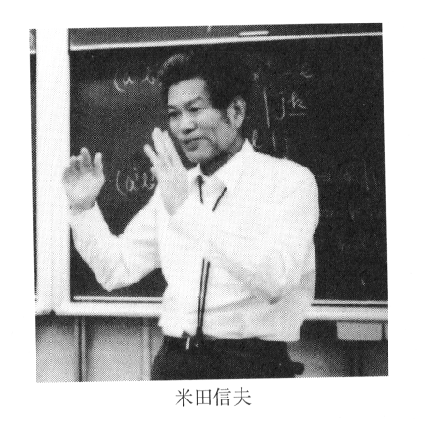
\includegraphics[width=.4\textwidth]{yoneda.png}\\
	\Huge Thanks!
\end{frame}
\end{document}